%\chapter{Bahnplanung} 
\chapter{Implementierung der Via-Punkt Trajektorie}
%\section{Bahnplanungsansätze im Vergleich}
%\section{Analyse und Approximation der KUKA Bahnplanung}
%\section{Implementierung der Via-Punkt Trajektorie}
Die Berechnung der Bewegungsbahn erfolgt für alle sechs Gelenkwinkel $\theta_i$ nach demselben Ansatz, einem Polynom sechster Ordnung. 
%
\begin{align}
	\theta(t) &= a_0 + a_1t + a_2t^2 + a_3t^3 + a_4t^4 + a_5t^5  + a_6t^6 \\
	\dot{\theta}(t) &= a_1 + 2a_2t + 3a_3t^2 + 4a_4t^3 + 5a_5t^4  + 6a_6t^5\\
	\ddot{\theta}(t) &= 2a_2 + 6a_3t + 12a_4t^2 + 20a_5t^3  + 30a_6t^4
\end{align}
%
Maßgeblich für die Ordnung des Polynoms ist die Anzahl von sieben Nebenbedingungen.  Definiert sind der Startwinkel $\theta_i(t_s)$, die Anfangsgeschwindigkeit $\dot{\theta}_i(t_s) = 0$, die Anfangsbeschleunigung $\ddot{\theta}_i(t_s) = 0$, der Via-Punkt-Winkel $\theta_i(t_v)$, sowie der Winkel im Zielpunkt $\theta_i(t_e)$, die Endgeschwindigkeit $\dot{\theta}_i(t_e) = 0$ und die Endbeschleunigung $\ddot{\theta}_i(t_e) = 0$. Darüber hinaus sind der Startzeitpunkt $t_s$, der Zeitpunkt für das Erreichen des Via-Punkts, sowie die Dauer der Bewegung über den Endzeitpunkt $t_e$ vorgegeben. 
%
Die Bestimmung der Parameter $a_0, ... a_6$ erfolgt durch Lösen des linearen Gleichungssystems \ref{eqn:lgs}. Die Implementierung in MATLAB\textsuperscript{\textregistered} ist im Anhang \ref{add:traj} hinterlegt.
%
\begin{equation}
	\label{eqn:lgs}
	\left[	\begin{matrix}
		1&\quad    t_s&\quad          	t_s^2&\quad              	t_s^3&\quad         	t_s^4&\quad              	t_s^5&\quad          	t_s^6\\
		0&\quad    t_s&\quad          	2t_s&\quad              	3t_s^2&\quad        	4t_s^3&\quad            	5t_s^4&\quad        	6t_s^5\\
		0&\quad    0&\quad         		2&\quad              	  	6t_s&\quad         	 	12t_s^2&\quad           	20t_s^3&\quad       	30t_s^4\\
		1&\quad    t_v&\quad         	t_v^2&\quad              	t_v^3&\quad         	t_v^4&\quad             	t_v^5&\quad          	t_v^6\\
		1&\quad    t_e&\quad        	t_e^2&\quad              	t_e^3&\quad          	t_e^4&\quad             	t_e^5&\quad          	t_e^6\\
		0&\quad    1&\quad   	   		2t_e&\quad              	3t_e^2&\quad        	4t_e^3&\quad           		5t_e^4&\quad        	6t_e^5\\   
		0&\quad    0&\quad          	2&\quad                 	6t_e&\quad          	12t_e^2&\quad           	20t_e^3&\quad       	30t_e^4
	\end{matrix}\right]
	\left[	\begin{matrix}
		a_0\\
		a_1\\
		a_2\\
		a_3\\
		a_4\\
		a_5\\
		a_6\\		
	\end{matrix}\right] = 
		\left[	\begin{matrix}
		\theta_s\\
		\dot{\theta}_s\\
		\ddot{\theta}_s\\
		\theta_v\\
		\theta_e\\
		\dot{\theta}_e\\
		\ddot{\theta}_e\\		
	\end{matrix}\right]
\end{equation}
%
Die Bestimmung der Roboterdynamik setzt voraus, dass die simulierte Bewegungsbahn $\theta(t)$, inklusive die zeitlichen Verläufe von $\dot{\theta}(t), ~\ddot{\theta}(t)$  die, von der KUKA Robotersteuerung berechnete Bahnverläufen möglichst genau approximieren. Hierzu wird eine Bewegung aus dem Programm $Kleben-Seitenwand$, welches auf der KRC5 des Roboters abgelegt ist und bereits für den Roboter auf Kollisionsfreiheit validiert ist, getestet. Die Bewegung ist in der Bewegungsart  Punkt-zu-Punkt (Point-To-Point)(PTP)) programmiert und sieht vor, den Roboter von dem letzten Prozesspunkt auf seine Warteposition (Home-Position) zu verfahren. Tabelle \ref{tab:simu} definiert die vorgegebenen Winkel. Die MATLAB\textsuperscript{\textregistered}-Implementierung der Bewegung im Anhang \ref{add:sim} hinterlegt.
\\
\begin{table}
\centering
\begin{tabular}{|c|c|c|}
	\hline
	Startwert Gelenkwinkel&  Zielwert Gelenkwinkel&  Via-Punkte\\
	\hline
	$\theta_{s1} = -53,8$&  $\theta_{e1} = -7,6^{\circ}$  &$\theta_{v1}$ = $\tfrac{\theta_{s1}+\theta_{e1}}{2}$  \\
	\hline
	$\theta_{s2} = -70,3^{\circ}$&  $\theta_{e2} = -119,3^{\circ}$    &$\theta_{v2}$ = $\tfrac{\theta_{s2}+\theta_{e2}}{2}$  \\
	\hline
	$\theta_{s3} = 98,8^{\circ}$&  $\theta_{e3} = 88,5^{\circ}$&$\theta_{v3}$ = $\tfrac{\theta_{s3}+\theta_{e3}}{2}$  \\
	\hline
	$\theta_{s4} = -69,9^{\circ}$&  $\theta_{e4} = 10,3^{\circ}$&$\theta_{v4}$ = $\tfrac{\theta_{s4}+\theta_{e4}}{2}$  \\
	\hline
	$\theta_{s5} = -58,7^{\circ}$&  $\theta_{e5} = 32,4^{\circ}$  &$\theta_{v5}$ = $\tfrac{\theta_{s5}+\theta_{e5}}{2}$  \\
	\hline
	$\theta_{s6} = 55,7^{\circ}$&  $\theta_{e6} = -10,2^{\circ}$&$\theta_{v6}$ = $\tfrac{\theta_{s6}+\theta_{e6}}{2}$  \\
	\hline
\end{tabular}
\caption{Winkelangaben letzter Prozesspunkt und Home-Position PRG $Kleben-Seitenwand$}
\label{tab:simu}
\end{table}
\\
Abbildung \ref{fig:gelenkwinkel}  visualisiert den simulierten  Verlauf der Gelenkwinkel. Abbildung \ref{fig:gelenkwinkelpy} zeigt den zeitlichen Verlauf der Gelenkwinkel am realen System. Die Daten sind mit einem einem  Zeitabstand $\Delta t = 4~\text{ms}$ abgetastet. Zur Visualisierung der Winkelgeschwindigkeit  erfolgt zunächst die Bildung des Differenzenquotienten für zwei benachbarte Abtastwerte. Durch eine anschießende Tiefpassfilterung wird der zeitliche Verlauf geglättet, siehe Abbildung \ref{fig:winkelgeschwindigkeit_py1}. Die Abtastfrequenz beträgt 250 Hz. Die Eckfrequenz des Butterworth-Filters wird auf 10 Hz definiert. Die Daten der Winkelbeschleunigung werden für dasselbe Vorgehen durch Anwendung des zentralen Differenzenquotienten für die zweite Ableitung berechnet. Der zeitliche Verlauf der Gelenkwinkel ist näherungsweise identisch. Da der Via-Punkt in der Simulation im Mittel zwischen den Start- und Zielpunkten und damit auf der Originalbahn definiert ist, wurde die Bewegung am realen Roboter ohne Definition des initialen Via-Punts gefahren. Der Verlauf der Beschleunigung ist detaillierter zu betrachten. Die Maximalwerte der Winkelbeschleunigung aller sechs Gelenke fallen in der simulierten Bewegung während den ersten zwei Beschleunigungsphasen circa 10-20 Prozent höher aus als die berechneten Beschleunigungen des realen Systems. Mithilfe der Originaldaten vor Anwendung der TP-Filterung wurde verifiziert, dass der Filteransatz keine Auswirkung auf die Maxima nimmt. Während der dritten und vierten Beschleunigungsphase sind die Maximalbeschleunigungen in den ersten drei Gelenken nahezu identisch. Aufgrund der hohen  Massen der ersten drei Verbindungsglieder bzw. Armelemente sind diese Werte von hoher Relevanz. Qualitativ ist im Beschleunigungsverlauf des realen Systems ein höherer Ruck beim Anfahren und Abbremsen erkennbar. Der Nulldurchgang der Beschleunigung und damit der Zeitpunkt der maximalen Geschwindigkeit (Zeitpunkt bei Erreichen des Via-Punkts) wird in der Simulation ca. 0,3 s eher erreicht. In der Schlussfolgerung wird bewertet, dass die Bewegungsbahn ausreichend genau simuliert wird, um die Parameter  $\theta(t), ~\dot{\theta}(t), ~\ddot{\theta}(t)$ dem RNEA zu übergeben. 

%
\newpage
\begin{figure}[]
	\centering
	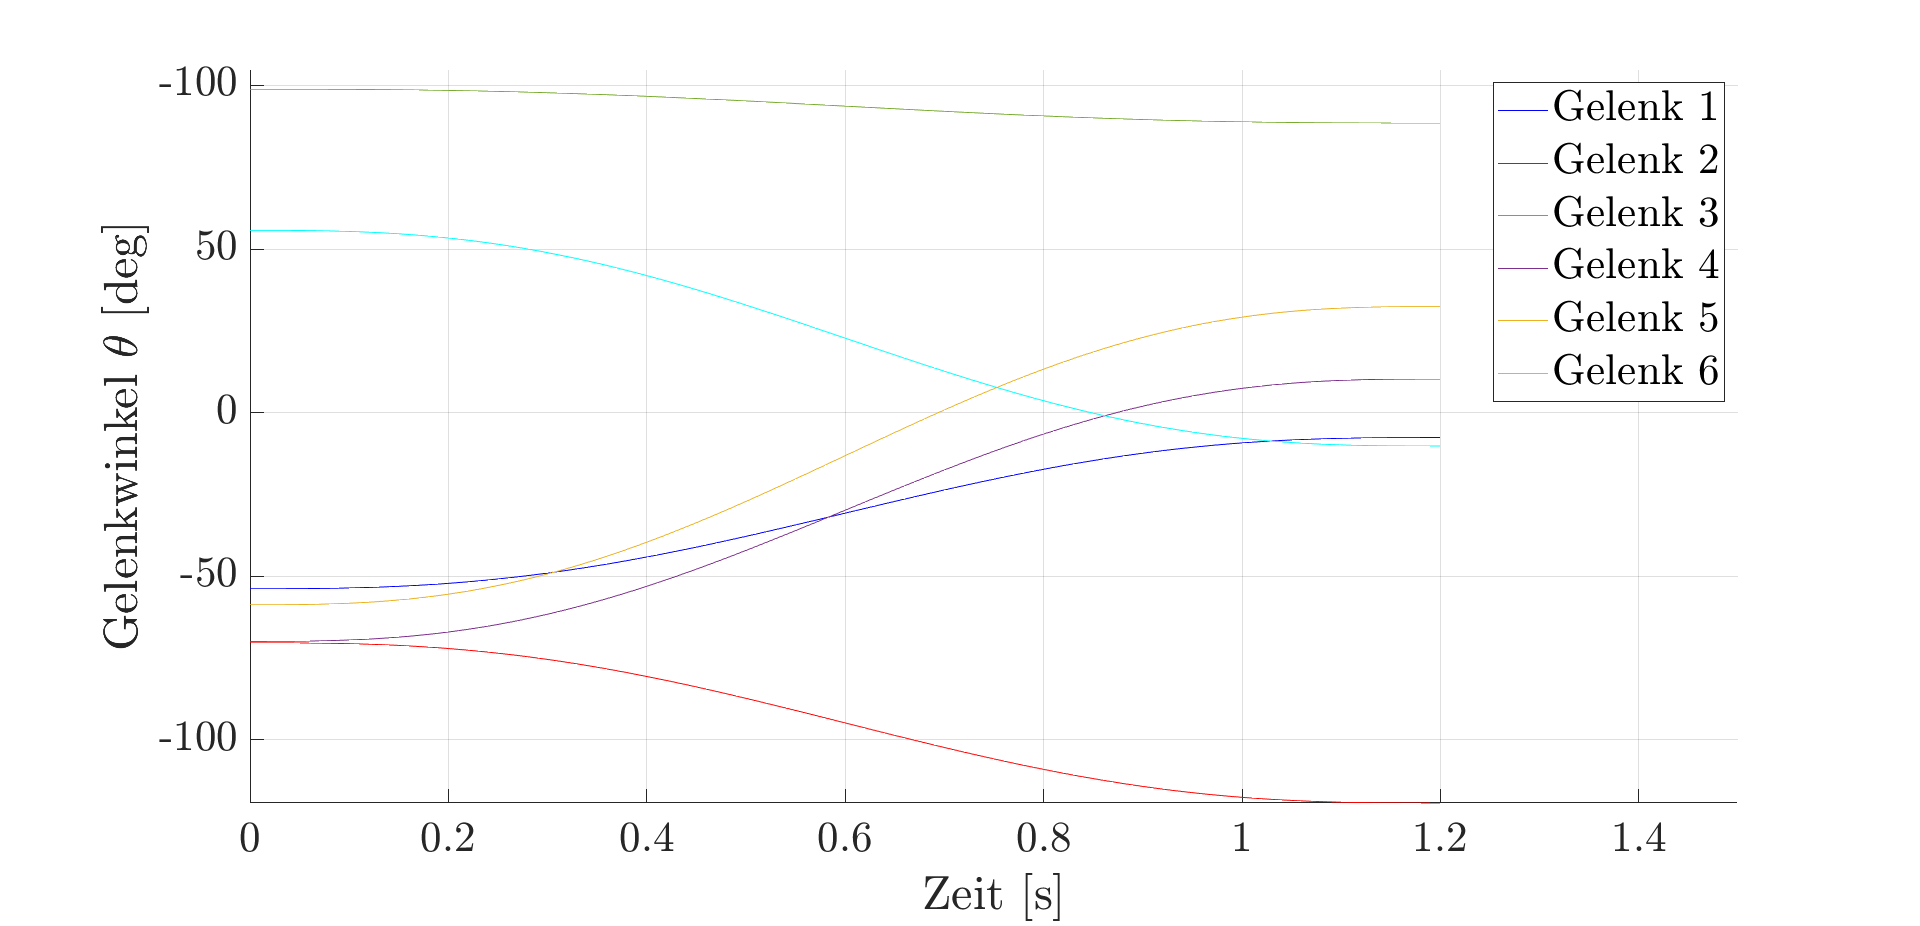
\includegraphics[width=1\linewidth]{images/gelenkwinkel}
	\caption{Gelenkwinkel}
	\label{fig:gelenkwinkel}
\end{figure}
%
\begin{figure}[]
	\centering
	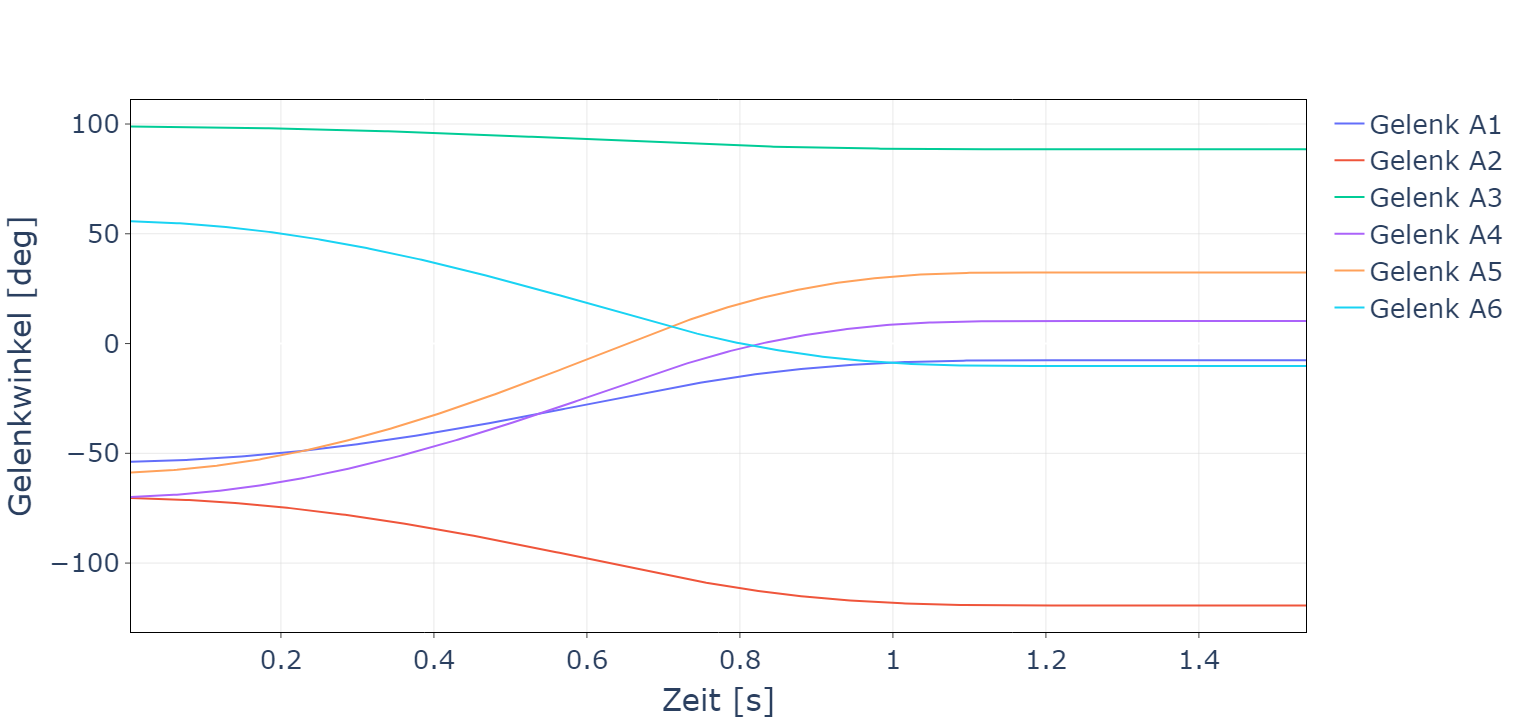
\includegraphics[width=1\linewidth]{images/gelenkwinkel_py}
	\caption{Gelenkwinkel}
	\label{fig:gelenkwinkelpy}
\end{figure}
%
\newpage
\begin{figure}[]
	\centering
	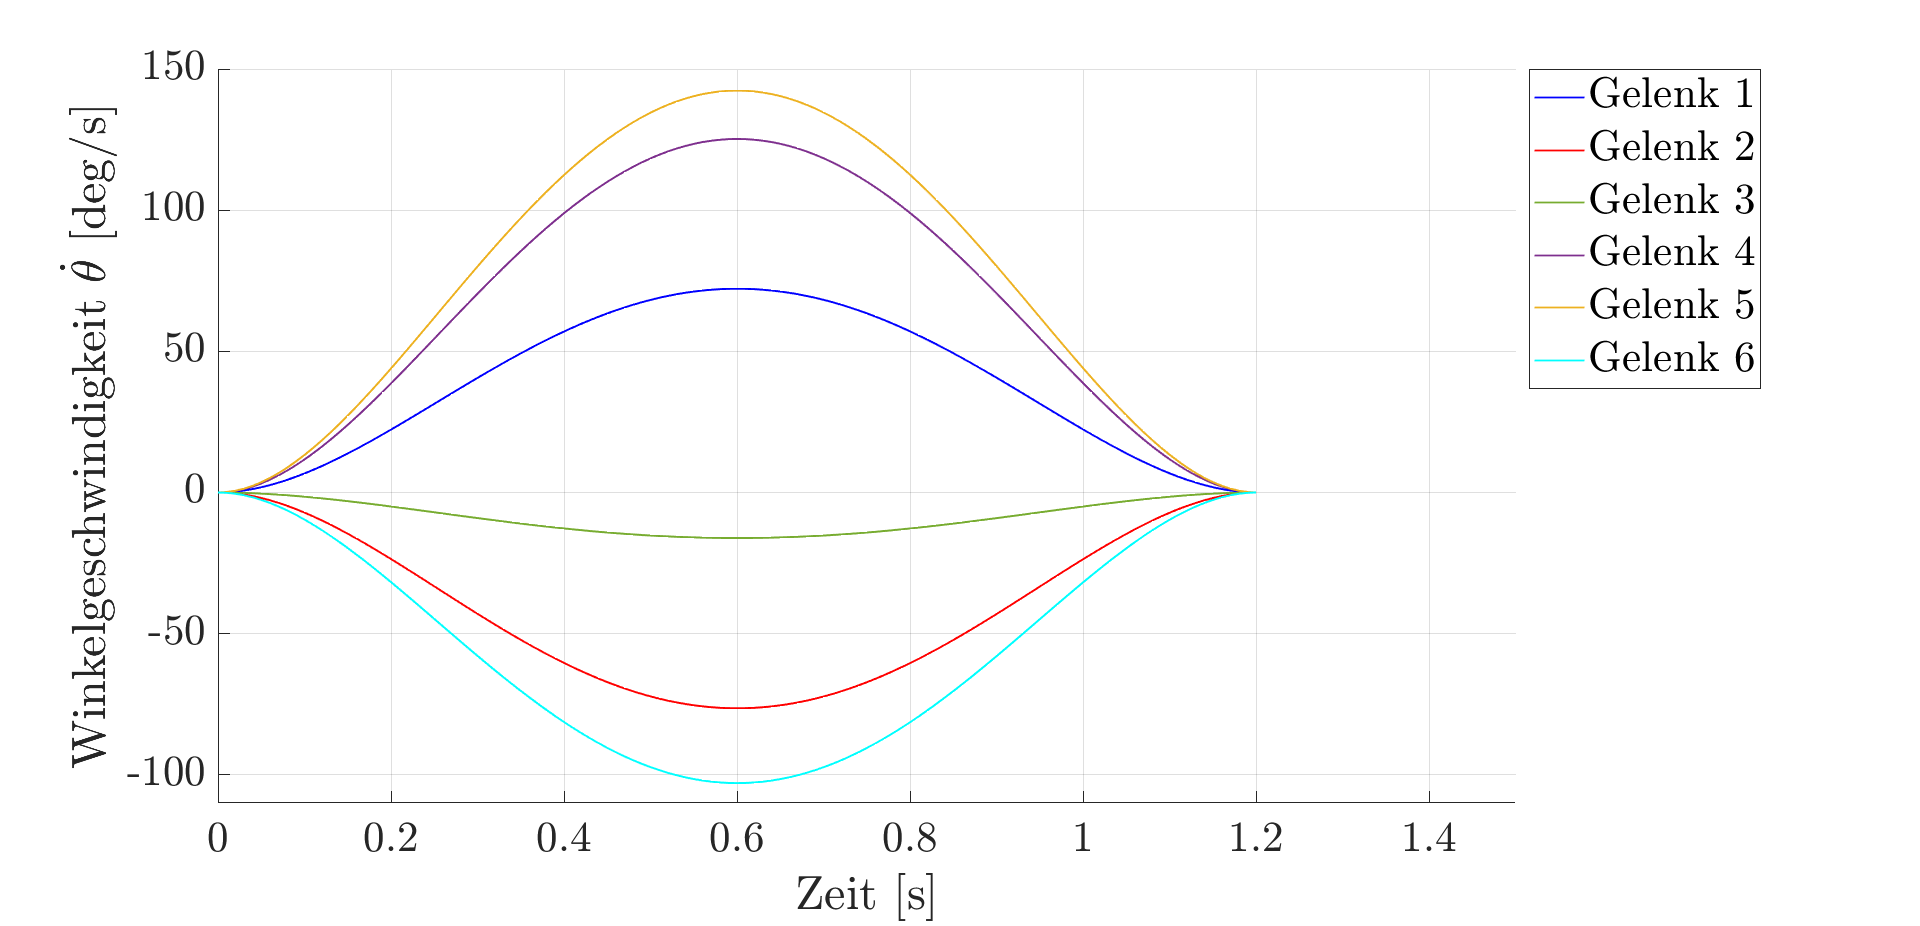
\includegraphics[width=1\linewidth]{images/winkelgeschwindigkeit}
	\caption{Winkelgeschwindigkeit}
	\label{fig:winkelgeschwindigkeit}
\end{figure}
%
\begin{figure}[]
	\centering
	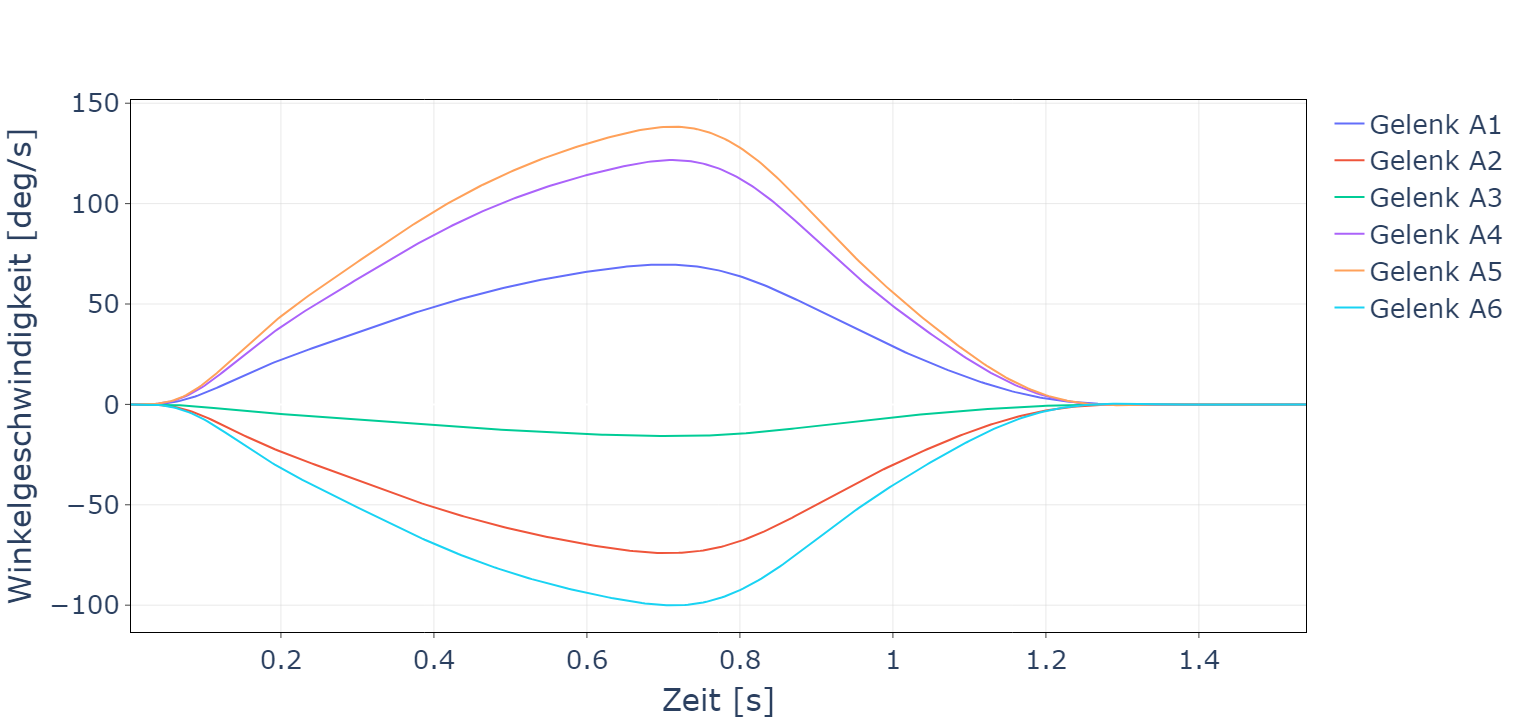
\includegraphics[width=1\linewidth]{images/winkelgeschwindigkeit_py}
	\caption{Winkelgeschwindigkeit}
	\label{fig:winkelgeschwindigkeit_py1}
\end{figure}
%
\newpage
\begin{figure}[]
	\centering
	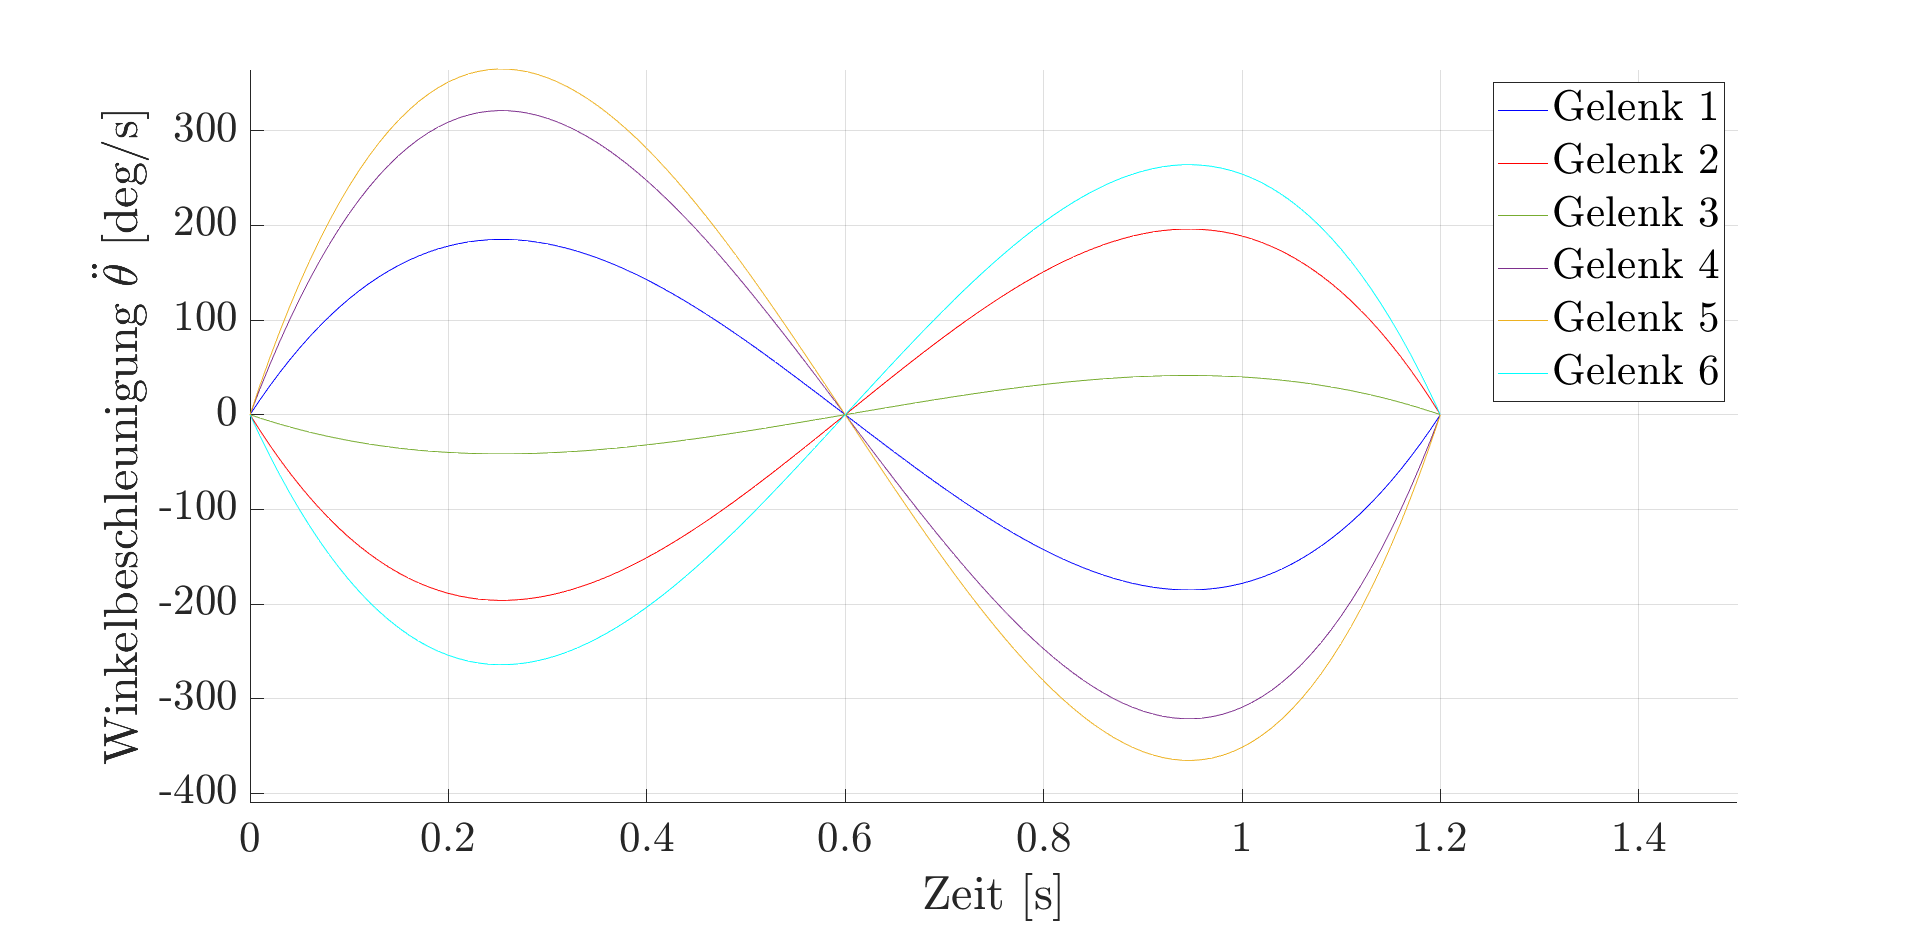
\includegraphics[width=1\linewidth]{images/winkelbeschleunigung}
	\caption{Winkelbeschleunigung}
	\label{fig:winkelbeschleunigung}
\end{figure}
%
\begin{figure}[]
	\centering
	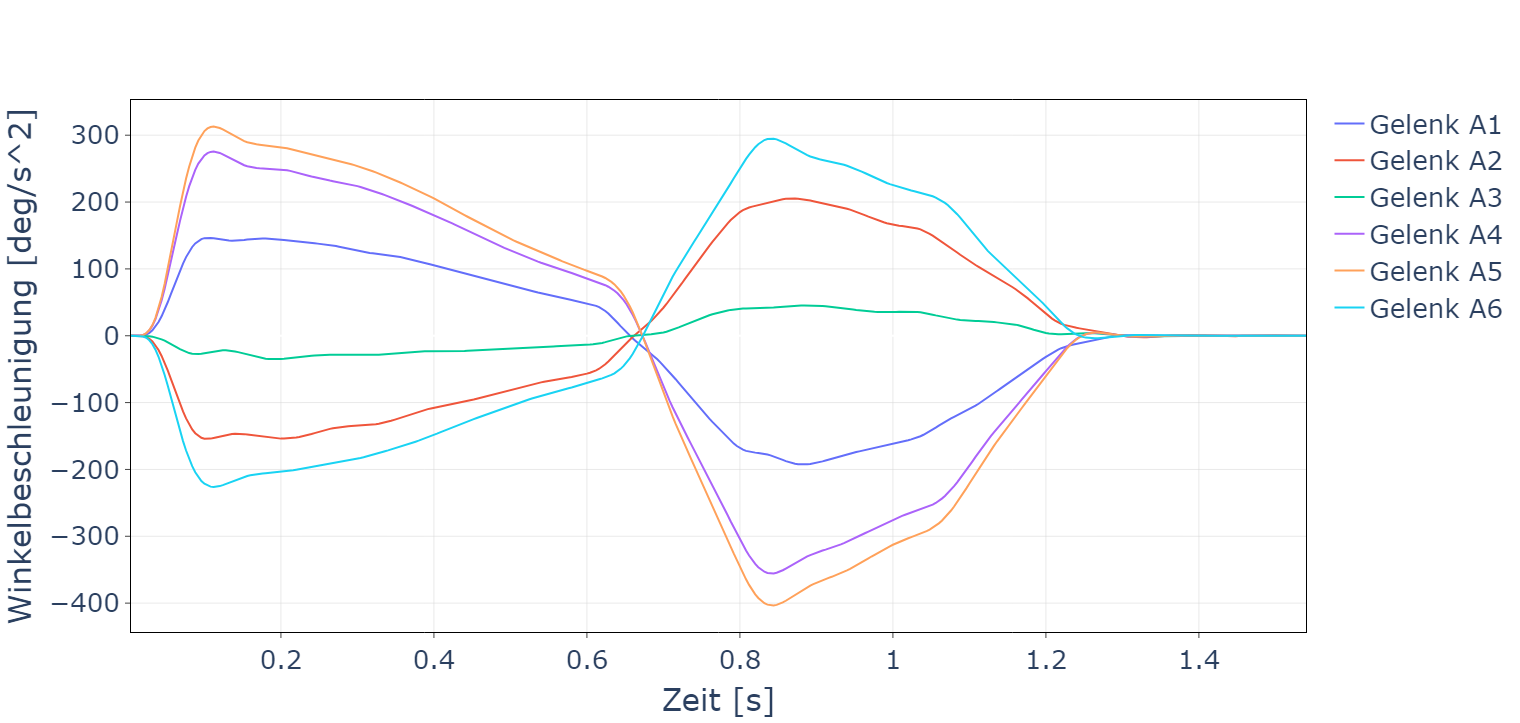
\includegraphics[width=1\linewidth]{images/winkelbeschleunigung_py1}
	\caption{Winkelbeschleunigung}
	\label{fig:winkelbeschleunigung_py}
\end{figure}
